% !BIB TS-program = biber
\documentclass[a4paper,oneside,12pt]{article}
\usepackage{BUPTthesisbachelor}
\usepackage{setspace}
\usepackage{graphicx}

\usepackage[final]{pdfpages}

\usepackage{listings}
\usepackage{xcolor}
\usepackage{setspace}
\usepackage{CJK}         % CJK 中文支持
\usepackage{fancyhdr}
\usepackage{amsmath,amsfonts,amssymb,graphicx}    % EPS 图片支持
\usepackage{subfigure}   % 使用子图形
\usepackage{indentfirst} % 中文段落首行缩进
\usepackage{bm}          % 公式中的粗体字符(用命令\boldsymbol)
\usepackage{multicol}    % 正文双栏
\usepackage{verbatim}
\usepackage{abstract} 

\usepackage{amssymb}
\usepackage{bm}
\usepackage{fontspec}

\usepackage{algorithm}  
\usepackage{algorithmicx}  
\usepackage{algpseudocode}

\usepackage{graphicx}


\lstdefinestyle{sharpc}{language=[Sharp]C, frame=lrtb, rulecolor=\color{blue!80!black}}

\title{\huge{The Description of Project}}
\author{Name: Xi Jingwei  \quad Student ID:517030910116 \quad   Email:jingweixi@sjtu.edu.cn}
\date{}  % 这一行用来去掉默认的日期显示
%%%%%%%%%%%%%%%%%%%%%%%%% Begin Documents %%%%%%%%%%%%%%%%%%%%%%%%%%
%中文摘要

\begin{document}
\maketitle
\setlength{\oddsidemargin}{0.5cm}
\setlength{\evensidemargin}{\oddsidemargin}
\setlength{\textwidth}{15cm}
\vspace{-.8cm}


%%%%%%%%%%%%%%%%%%%%%%%%%%%%%%%%%%%%%%%%%%%%%%%%%%%%%%%%%%%%%%%%%%%%%
%                                                                  %
%   Copyright (c) 2010 - 2011 Caspar Zhang <casparant@gmail.com>   %
%                                                                  %
%   This copyrighted material is made available to anyone wishing  %
%   to use, modify, copy, or redistribute it subject to the terms  %
%   and conditions of the GNU General Public License version 2.    %
%                                                                  %
%   This program is distributed in the hope that it will be        %
%   useful, but WITHOUT ANY WARRANTY; without even the implied     %
%   warranty of MERCHANTABILITY or FITNESS FOR A PARTICULAR        %
%   PURPOSE. See the GNU General Public License for more details.  %
%                                                                  %
%   You should have received a copy of the GNU General Public      %
%   License along with this program; if not, write to the Free     %
%   Software Foundation, Inc., 51 Franklin Street, Fifth Floor,    %
%   Boston, MA 02110-1301, USA.                                    %
%                                                                  %
%%%%%%%%%%%%%%%%%%%%%%%%%%%%%%%%%%%%%%%%%%%%%%%%%%%%%%%%%%%%%%%%%%%%

% 你只需要修改下面几行就可以完成大部分内容的填写,
% 这要求你具有一定的LaTeX基础,但是如果你足够聪明,
% 不具有LaTeX基础也可以完成。

% 论文中文题目
\def\thesistitle{
大学生使用MOOC的影响因素研究}

\def\author{
席经纬}

    % Main ?????????????????????????????????????????items 
%%%%%%%%%%%%%%%%%%%%%%%%%%%%%%%%%%%%%%%%%%%%%%%%%%%%%%%%%%%%%%%%%%%%%
%                                                                  %
%   Modified by Bing Hsu <hello@antinucleon.com> 2013              %
%   Forked From (c) 2010 - 2011 Caspar Zhang <casparant@gmail.com> %
%                                                                  %
%   This copyrighted material is made available to anyone wishing  %
%   to use, modify, copy, or redistribute it subject to the terms  %
%   and conditions of the GNU General Public License version 2.    %
%                                                                  %
%   This program is distributed in the hope that it will be        %
%   useful, but WITHOUT ANY WARRANTY; without even the implied     %
%   warranty of MERCHANTABILITY or FITNESS FOR A PARTICULAR        %
%   PURPOSE. See the GNU General Public License for more details.  %
%                                                                  %
%   You should have received a copy of the GNU General Public      %
%   License along with this program; if not, write to the Free     %
%   Software Foundation, Inc., 51 Franklin Street, Fifth Floor,    %
%   Boston, MA 02110-1301, USA.                                    %
%                                                                  %
%%%%%%%%%%%%%%%%%%%%%%%%%%%%%%%%%%%%%%%%%%%%%%%%%%%%%%%%%%%%%%%%%%%%

%%%%%%%%%%%%%%%%%%%%%%%%%%%%%%%%%%%%%%%%%%%%%%%%%%%%%%%%%%%%%%%%%%%%
%                                                                  %
%   Copyright (c) 2010 - 2011 Caspar Zhang <casparant@gmail.com>   %
%                                                                  %
%   This copyrighted material is made available to anyone wishing  %
%   to use, modify, copy, or redistribute it subject to the terms  %
%   and conditions of the GNU General Public License version 2.    %
%                                                                  %
%   This program is distributed in the hope that it will be        %
%   useful, but WITHOUT ANY WARRANTY; without even the implied     %
%   warranty of MERCHANTABILITY or FITNESS FOR A PARTICULAR        %
%   PURPOSE. See the GNU General Public License for more details.  %
%                                                                  %
%   You should have received a copy of the GNU General Public      %
%   License along with this program; if not, write to the Free     %
%   Software Foundation, Inc., 51 Franklin Street, Fifth Floor,    %
%   Boston, MA 02110-1301, USA.                                    %
%                                                                  %
%%%%%%%%%%%%%%%%%%%%%%%%%%%%%%%%%%%%%%%%%%%%%%%%%%%%%%%%%%%%%%%%%%%%

% 你只需要修改下面内容就可以完成中英文摘要,
% 这要求你具有一定的LaTeX基础,但是还是那句话,
% 如果你足够聪明,不具有LaTeX基础也可以完成。

% 中文摘要
\def\abstractcn{
%从这里开始写你的摘要,分段需要空一行。
以MOOC为主的在线教育平台席卷全球,而当前国内外对于MOOC学习的主要群体——高校大学生的学习行为研究较少。经过
观察,大学生多是在上大学之后才开始使用MOOC,而在大学之前的学习阶段不曾使用MOOC进行学习。本文自编调查问卷,
并进行了样本特征分析、信度分析、效度检验。根据问卷调查分析
统计,文章总结出影响大学生在上大学前就开始使用MOOC的影响因素
主要有家庭经济状况、高中所在学校的性质、母亲受教育程度、父亲受教育程度。
通过对这四个影响因素的权重分析,文章指出家庭经济状况和高中学校性质
对大学生在上大学前就开始使用MOOC的影响较大。最后,文章对得出的结果进行分析,提出一些增加MOOC在中小学生群体中
使用情况的建议,以期让更多的学习者受益于优质的MOOC课程资源。


%摘要结束
}
\def\abstractcns{
随着信息技术的快速发展,教育技术也在不断变革,并给教育带来新的变化。MOOC以互联网为载体,将全球顶级大学的
优质课程资源,以极低的成本传递到原本无法取得这些资源的 世界各地学习者的终端设备上,使他们随时随地获取最优
质的学习资源。此外,MOOC学习者 可以根据时间、能力自行把握学习进度,选择学习环境,充分体现了“自主学习”的理念。

据教育部在线教育研究中心发布的《2016 中国慕课行业研究白皮书》预计,2016年中国MOOC学习者将超过 1000 万,
MOOC学习者数量呈现出快速增长趋势[。然而,尽管MOOC蓬勃发展、用户数量持续增多,但相关研究显示,MOOC的使用
者主要为高校大学生,很少的部分为中小学生。为此,本研究采用问卷调查、主成分分析等研究方法,对影响大学生在上大学前
就开始使用MOOC的影响因素进行研究,并在此基础上,提出一些增加MOOC在中小学生群体中
使用情况的建议。
}

% 中文关键字 
% TODO: 改成可变长度的
\def\abscnkeyone{MOOC}
\def\abscnkeytwo{数据分析}
\def\abscnkeythree{大学生}



% 中文摘要
\begin{titlepage}
    \begin{spacing}{1.05}
        \centering
        \parbox[c]{.6\textwidth}{\thesistitlefont{\thesistitle}}
    \end{spacing}

    \begin{spacing}{1.6}
        \centering
        \sanhao\quad{} \\ 
        \abscnname{517030910116\quad{}\quad{}\quad{}席经纬\quad{}\quad{}\quad{}\quad{}F1703301} \\ 
        \xiaosanhao\quad{}
    \end{spacing}


    \begin{spacing}{0.8}
        \centering
        \sanhao\quad{} \\ 
        \abscnname{摘\quad{}要} \\ 
        \xiaosanhao\quad{}
    \end{spacing}
    
    \normalsize

    \abstractcn
    
    \quad{}

    \abscnkey{关键词}\quad{}%
    \abscnkeys{\abscnkeyone\quad{}%
                      \abscnkeytwo\quad{}%
                      \abscnkeythree\quad{}%
                      }%

    \begin{spacing}{1.6}
        \centering
        \sanhao\quad{} \\ 
        \abscnname{引\quad{}言} \\ 
        \xiaosanhao\quad{}
    \end{spacing}
    
    \normalsize

    \abstractcns
    
    \quad{}

\end{titlepage}
  % Abstract
%%%%%%%%%%%%%%%%%%%%%%%%%%%%% Main Area %%%%%%%%%%%%%%%%%%%%%%%%%%%%
\setlength{\oddsidemargin}{-.5cm}  % 3.17cm - 1 inch
\setlength{\evensidemargin}{\oddsidemargin}
\setlength{\textwidth}{17.00cm}

\section{Problem1}
\subsection{Files}
\subsubsection{ptree.c}
Function static int ptree(struct prinfo *buf, int *nr)

Call function $dfs$ and use read\_lock and read\_unlock to protect the data.Then copy data from task[] to buf.

Function void $dfs$(struct task\_struct start, int deep)

Search all processes and store information in $dfs$ order.

\subsubsection{Makefile}

Use Makefile to compile the ptree.c file.

\subsection{Process}

a. I searched a lot of information of task\_struct and list function in Linux kernel on the internet. Then I know how to use the function list\_entry and list\_for\_each.

b. When I coded the $dfs$ function, I met many problems. I don't know how to depth-first-search a tree without knowing all the children of parent. Then I search on Google and I find node -> children will point to the head of children list. And I use list\_for\_each function to depth-first-search the process tree.

c. At problem1, I don't know the difference between struct task\_struct and list\_head. And I didn't know how to transfer them. With the help of friends, I learn to use list\_entry((\&node , struct task\_struct, sibling) to transfer them.




\section{Problem2}
\subsection{Files}
\subsubsection{ptree.c}

The program will call ptree function in kernel and print the entire process tree (in DFS order) using tabs to indent children with respect to their parents.

\subsubsection{Android.mk}

The make file for project.

\subsection{Process}

At first, I used syscall 391 in the program, but I could not make it work in kernel and I can not find the problem. With the help of TAs, I changed syscall from 391 to 356 and then it worked. 

\subsection{Result}

\begin{lstlisting}
The number of task is 59!
Print start
swapper, 0, 0, 0, 1, 0, 0
	init, 1, 1, 0, 45, 2, 0
		ueventd, 45, 1, 1, 0, 61, 0
		logd, 61, 1, 1, 0, 62, 1036
		vold, 62, 1, 1, 0, 68, 0
		healthd, 68, 1, 1, 0, 69, 0
		lmkd, 69, 1, 1, 0, 70, 0
		servicemanager, 70, 1, 1, 0, 71, 1000
		surfaceflinger, 71, 1, 1, 0, 73, 1000
		qemud, 73, 1, 1, 0, 76, 0
		sh, 76, 1, 1, 0, 77, 2000
		adbd, 77, 1, 1, 197, 78, 0
			sh, 197, 1, 77, 370, 1, 0
				ptreeARM, 370, 0, 197, 0, 1, 0
		netd, 78, 1, 1, 371, 79, 0
			sh, 371, 0, 78, 0, 1, 0
		debuggerd, 79, 1, 1, 0, 80, 0
		rild, 80, 1, 1, 0, 81, 1001
		drmserver, 81, 1, 1, 0, 82, 1019
		mediaserver, 82, 1, 1, 0, 83, 1013
		installd, 83, 1, 1, 0, 84, 0
		keystore, 84, 1, 1, 0, 85, 1017
		main, 85, 1, 1, 235, 86, 0
			system_server, 235, 1, 85, 0, 1, 1000
		gatekeeperd, 86, 1, 1, 0, 89, 1000
		perfprofd, 89, 1, 1, 0, 90, 0
		fingerprintd, 90, 1, 1, 0, 122, 1000
		bootanimation, 122, 1, 1, 0, 1, 1003
	kthreadd, 2, 1, 0, 3, 0, 0
		ksoftirqd/0, 3, 1, 2, 0, 4, 0
		kworker/0:0, 4, 1, 2, 0, 5, 0
		kworker/u:0, 5, 1, 2, 0, 6, 0
		khelper, 6, 1, 2, 0, 7, 0
		sync_supers, 7, 1, 2, 0, 8, 0
		bdi-default, 8, 1, 2, 0, 9, 0
		kblockd, 9, 1, 2, 0, 10, 0
		rpciod, 10, 1, 2, 0, 11, 0
		kworker/0:1, 11, 1, 2, 0, 12, 0
		kswapd0, 12, 1, 2, 0, 13, 0
		fsnotify_mark, 13, 1, 2, 0, 14, 0
		crypto, 14, 1, 2, 0, 25, 0
		kworker/u:1, 25, 1, 2, 0, 30, 0
		mtdblock0, 30, 1, 2, 0, 35, 0
		mtdblock1, 35, 1, 2, 0, 40, 0
		mtdblock2, 40, 1, 2, 0, 41, 0
		binder, 41, 1, 2, 0, 42, 0
		deferwq, 42, 1, 2, 0, 43, 0
		kworker/u:2, 43, 1, 2, 0, 44, 0
		mmcqd/0, 44, 1, 2, 0, 47, 0
		jbd2/mtdblock0-, 47, 1, 2, 0, 48, 0
		ext4-dio-unwrit, 48, 1, 2, 0, 51, 0
		flush-31:1, 51, 1, 2, 0, 53, 0
		jbd2/mtdblock1-, 53, 1, 2, 0, 54, 0
		ext4-dio-unwrit, 54, 1, 2, 0, 57, 0
		flush-31:2, 57, 1, 2, 0, 59, 0
		jbd2/mtdblock2-, 59, 1, 2, 0, 60, 0
		ext4-dio-unwrit, 60, 1, 2, 0, 63, 0
		kworker/0:2, 63, 1, 2, 0, 94, 0
		kauditd, 94, 1, 2, 0, 0, 0
Print end


\end{lstlisting}

\section{Problem3}
\subsection{Files}
\subsubsection{process.c}

The program enerate a new process and output “StudentIDParent” with PID, then generates its children process output “StudentIDChild” with PID.

And in child process it will execute ptree.

\subsubsection{Android.mk}

The make file for project.

\subsection{Process}

I searched on the internet for how to get the process id, then I get know that getpid() function can get the id of process. And after searching the relationship of parent process and child process, I know the pid = fork() in parent process will return the child process id.

\subsection{Result}

\section{Problem3}
\subsection{Files}
\subsubsection{process.c}

The program enerate a new process and output “StudentIDParent” with PID, then generates its children process output “StudentIDChild” with PID.

And in child process it will execute ptree.

\subsubsection{Android.mk}

The make file for project.

\subsection{Process}

I searched on the internet for how to get the process id, then I get know that getpid() function can get the id of process. And after searching the relationship of parent process and child process, I know the pid = fork() in parent process will return the child process id.

\subsection{Result}

\begin{lstlisting}
517030910116 Parent pid = 701
517030910116 Child pid = 702
The number of task is 59!
Print start
swapper, 0, 0, 0, 1, 0, 0
	init, 1, 1, 0, 45, 2, 0
		ueventd, 45, 1, 1, 0, 61, 0
		logd, 61, 1, 1, 0, 62, 1036
		vold, 62, 1, 1, 0, 68, 0
		healthd, 68, 1, 1, 0, 69, 0
		lmkd, 69, 1, 1, 0, 70, 0
		servicemanager, 70, 1, 1, 0, 71, 1000
		surfaceflinger, 71, 1, 1, 0, 73, 1000
		qemud, 73, 1, 1, 0, 76, 0
		sh, 76, 1, 1, 0, 77, 2000
		adbd, 77, 1, 1, 197, 78, 0
			sh, 197, 1, 77, 370, 1, 0
				ptreeARM, 370, 0, 197, 0, 1, 0
		netd, 78, 1, 1, 371, 79, 0
			sh, 371, 0, 78, 0, 1, 0
		debuggerd, 79, 1, 1, 0, 80, 0
		rild, 80, 1, 1, 0, 81, 1001
		drmserver, 81, 1, 1, 0, 82, 1019
		mediaserver, 82, 1, 1, 0, 83, 1013
		installd, 83, 1, 1, 0, 84, 0
		keystore, 84, 1, 1, 0, 85, 1017
		main, 85, 1, 1, 235, 86, 0
			system_server, 235, 1, 85, 0, 1, 1000
		gatekeeperd, 86, 1, 1, 0, 89, 1000
		perfprofd, 89, 1, 1, 0, 90, 0
		fingerprintd, 90, 1, 1, 0, 122, 1000
		bootanimation, 122, 1, 1, 0, 1, 1003
	kthreadd, 2, 1, 0, 3, 0, 0
		ksoftirqd/0, 3, 1, 2, 0, 4, 0
		kworker/0:0, 4, 1, 2, 0, 5, 0
		kworker/u:0, 5, 1, 2, 0, 6, 0
		khelper, 6, 1, 2, 0, 7, 0
		sync_supers, 7, 1, 2, 0, 8, 0
		bdi-default, 8, 1, 2, 0, 9, 0
		kblockd, 9, 1, 2, 0, 10, 0
		rpciod, 10, 1, 2, 0, 11, 0
		kworker/0:1, 11, 1, 2, 0, 12, 0
		kswapd0, 12, 1, 2, 0, 13, 0
		fsnotify_mark, 13, 1, 2, 0, 14, 0
		crypto, 14, 1, 2, 0, 25, 0
		kworker/u:1, 25, 1, 2, 0, 30, 0
		mtdblock0, 30, 1, 2, 0, 35, 0
		mtdblock1, 35, 1, 2, 0, 40, 0
		mtdblock2, 40, 1, 2, 0, 41, 0
		binder, 41, 1, 2, 0, 42, 0
		deferwq, 42, 1, 2, 0, 43, 0
		kworker/u:2, 43, 1, 2, 0, 44, 0
		mmcqd/0, 44, 1, 2, 0, 47, 0
		jbd2/mtdblock0-, 47, 1, 2, 0, 48, 0
		ext4-dio-unwrit, 48, 1, 2, 0, 51, 0
		flush-31:1, 51, 1, 2, 0, 53, 0
		jbd2/mtdblock1-, 53, 1, 2, 0, 54, 0
		ext4-dio-unwrit, 54, 1, 2, 0, 57, 0
		flush-31:2, 57, 1, 2, 0, 59, 0
		jbd2/mtdblock2-, 59, 1, 2, 0, 60, 0
		ext4-dio-unwrit, 60, 1, 2, 0, 63, 0
		kworker/0:2, 63, 1, 2, 0, 94, 0
		kauditd, 94, 1, 2, 0, 0, 0
Print end

\end{lstlisting}
\section{Problem4}
\subsection{Files}
\subsubsection{server.c}

Function int main()

The server will listen to the port. If there is a client want to connect, it will connect to the client and create a new thread to call serve function.

Function void *serve(void *clientfd)

It will judge whether server could serve client or not. If the count of client that server served concurrently is less than two, the server can receive the client message and change it. Then it will send the message changed to the client.

\subsubsection{client.c}

The program client.c will send message to server and receive the message changed by server.

\subsection{Process}

1. I met a lot of problems in server problem. At first, I don't know the how to create thread and how to deal with critical section problem. I find answers on the internet and use pthread and mutex.

2. I use two mutex. One mutex is for variable count which is the number of client which are served by server. The other mutex is to make new coming clients to wait if there are two clients served concurrently.

\subsection{Result}

When client1 and client2 are served by server, client3 need to wait.

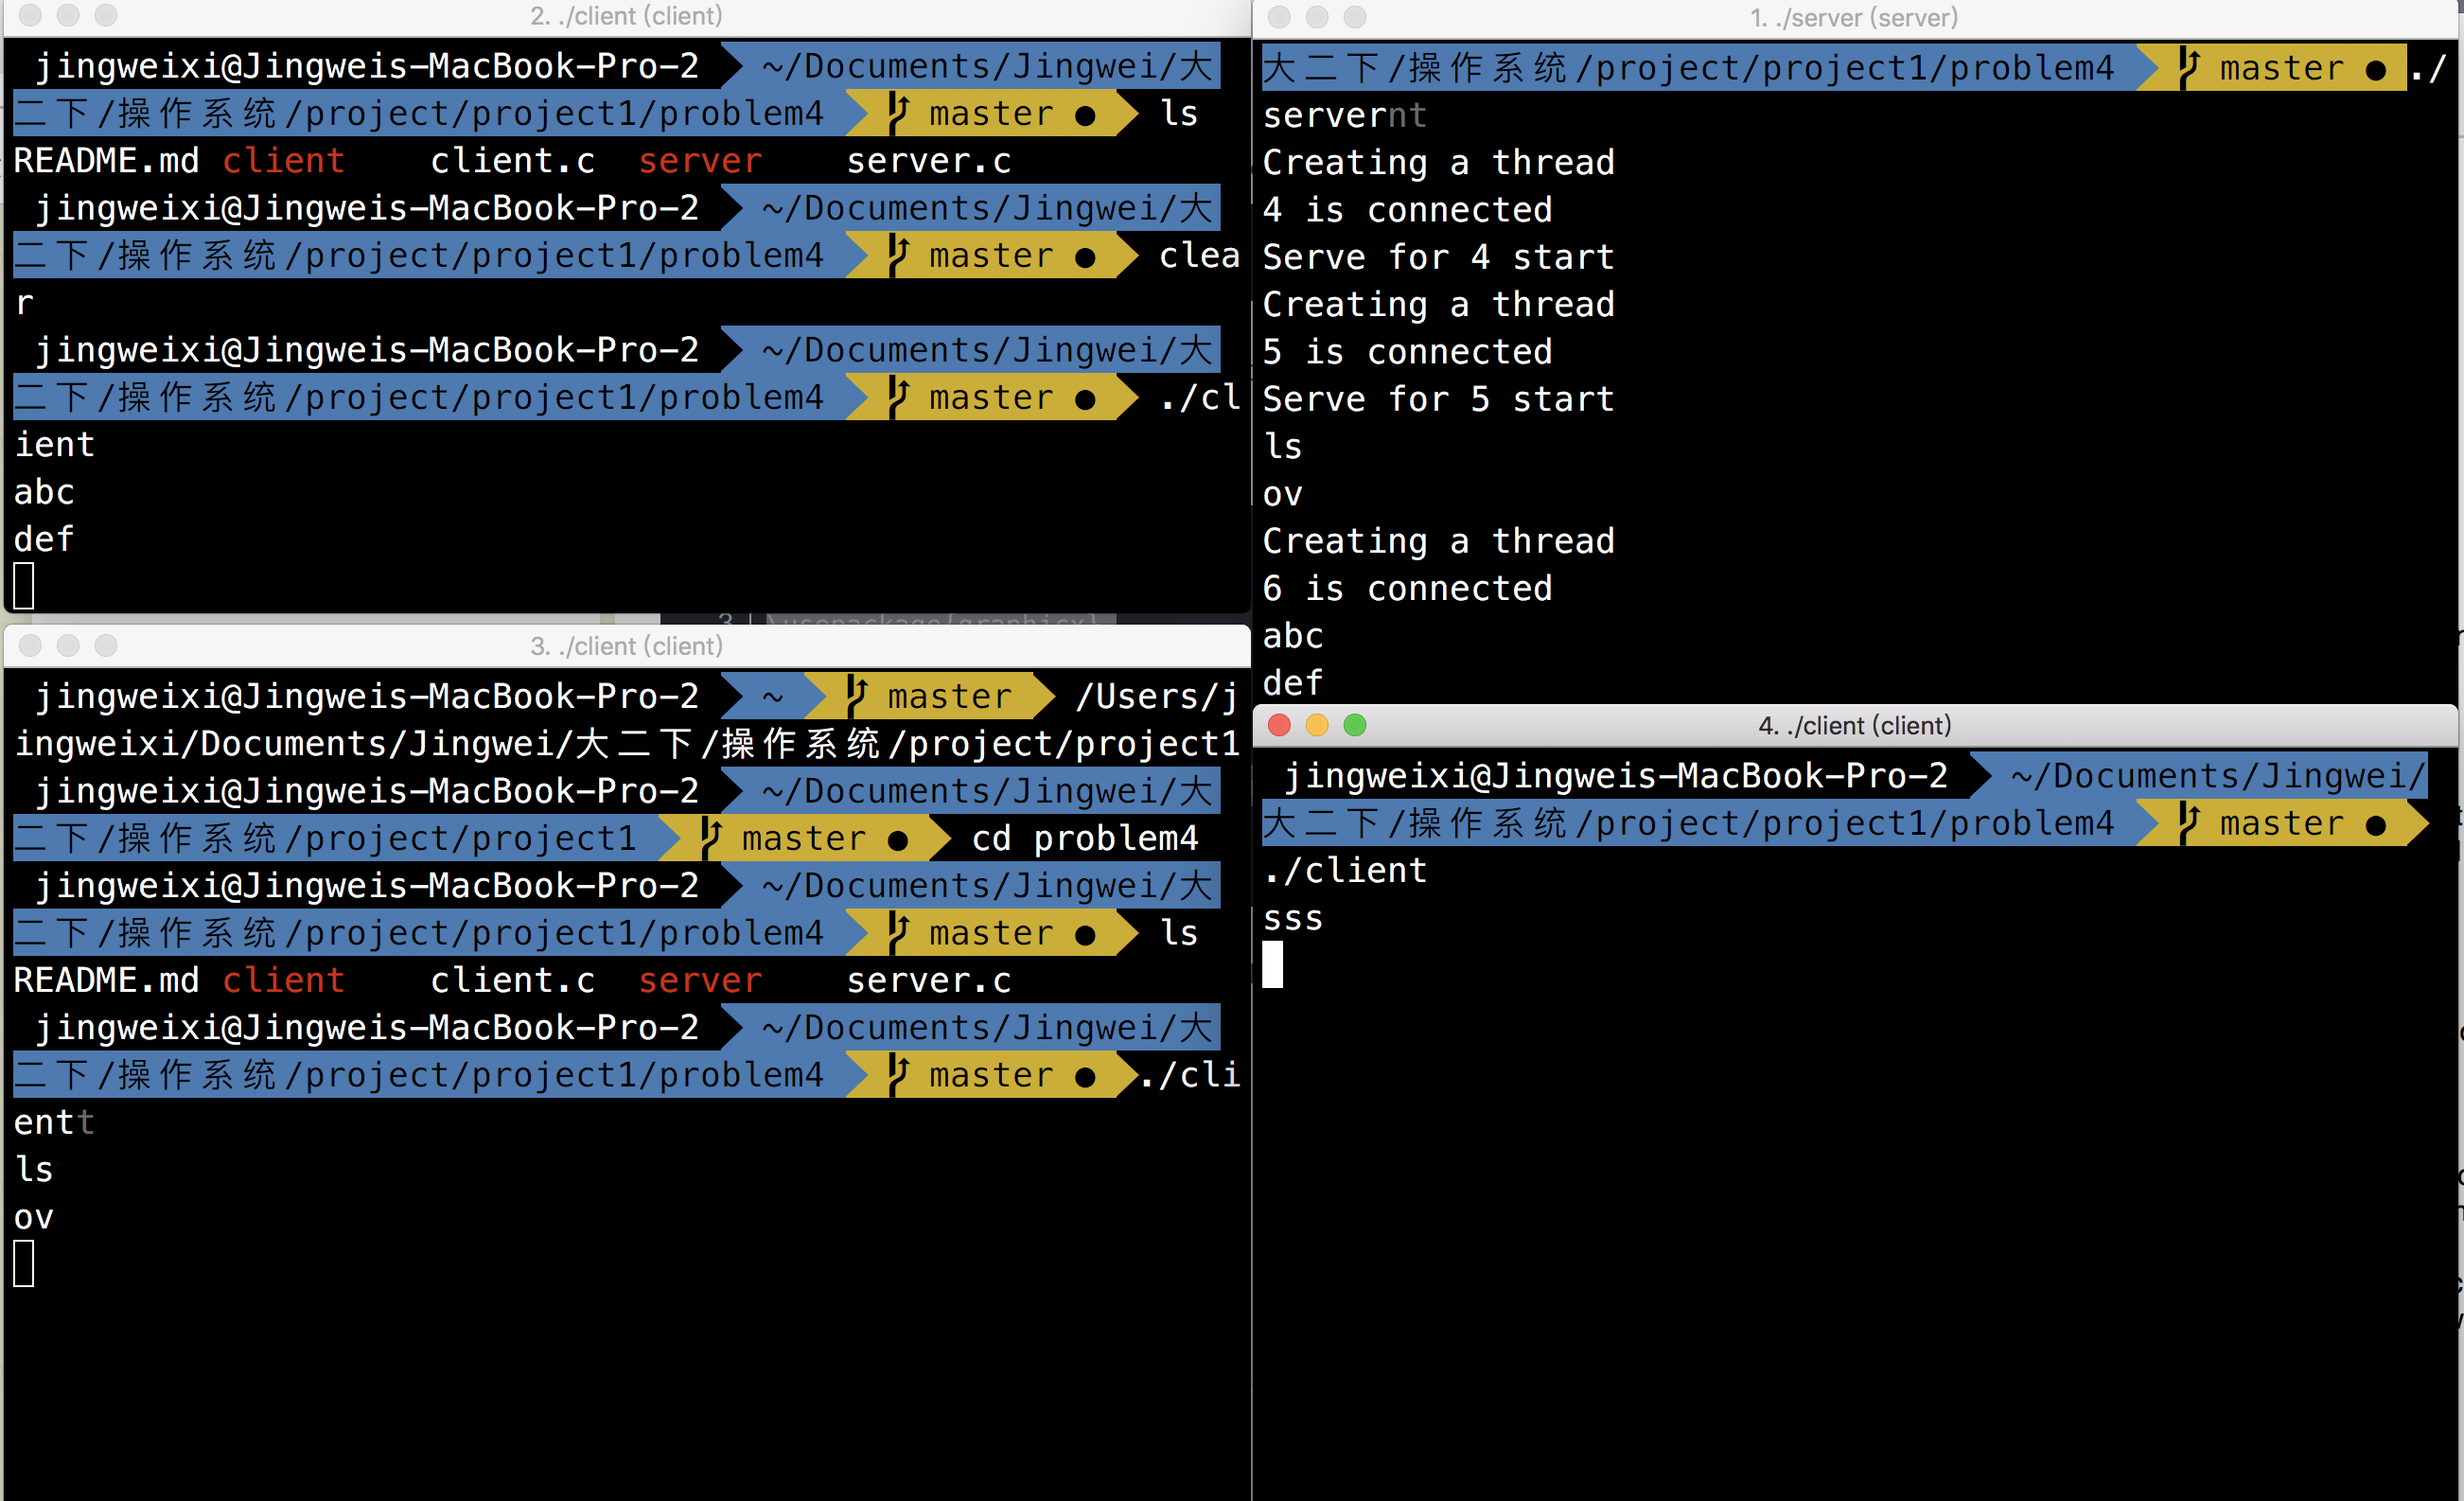
\includegraphics[scale=0.3]{1.png}

When client1 quit and end the service, the client3 will be served by server.

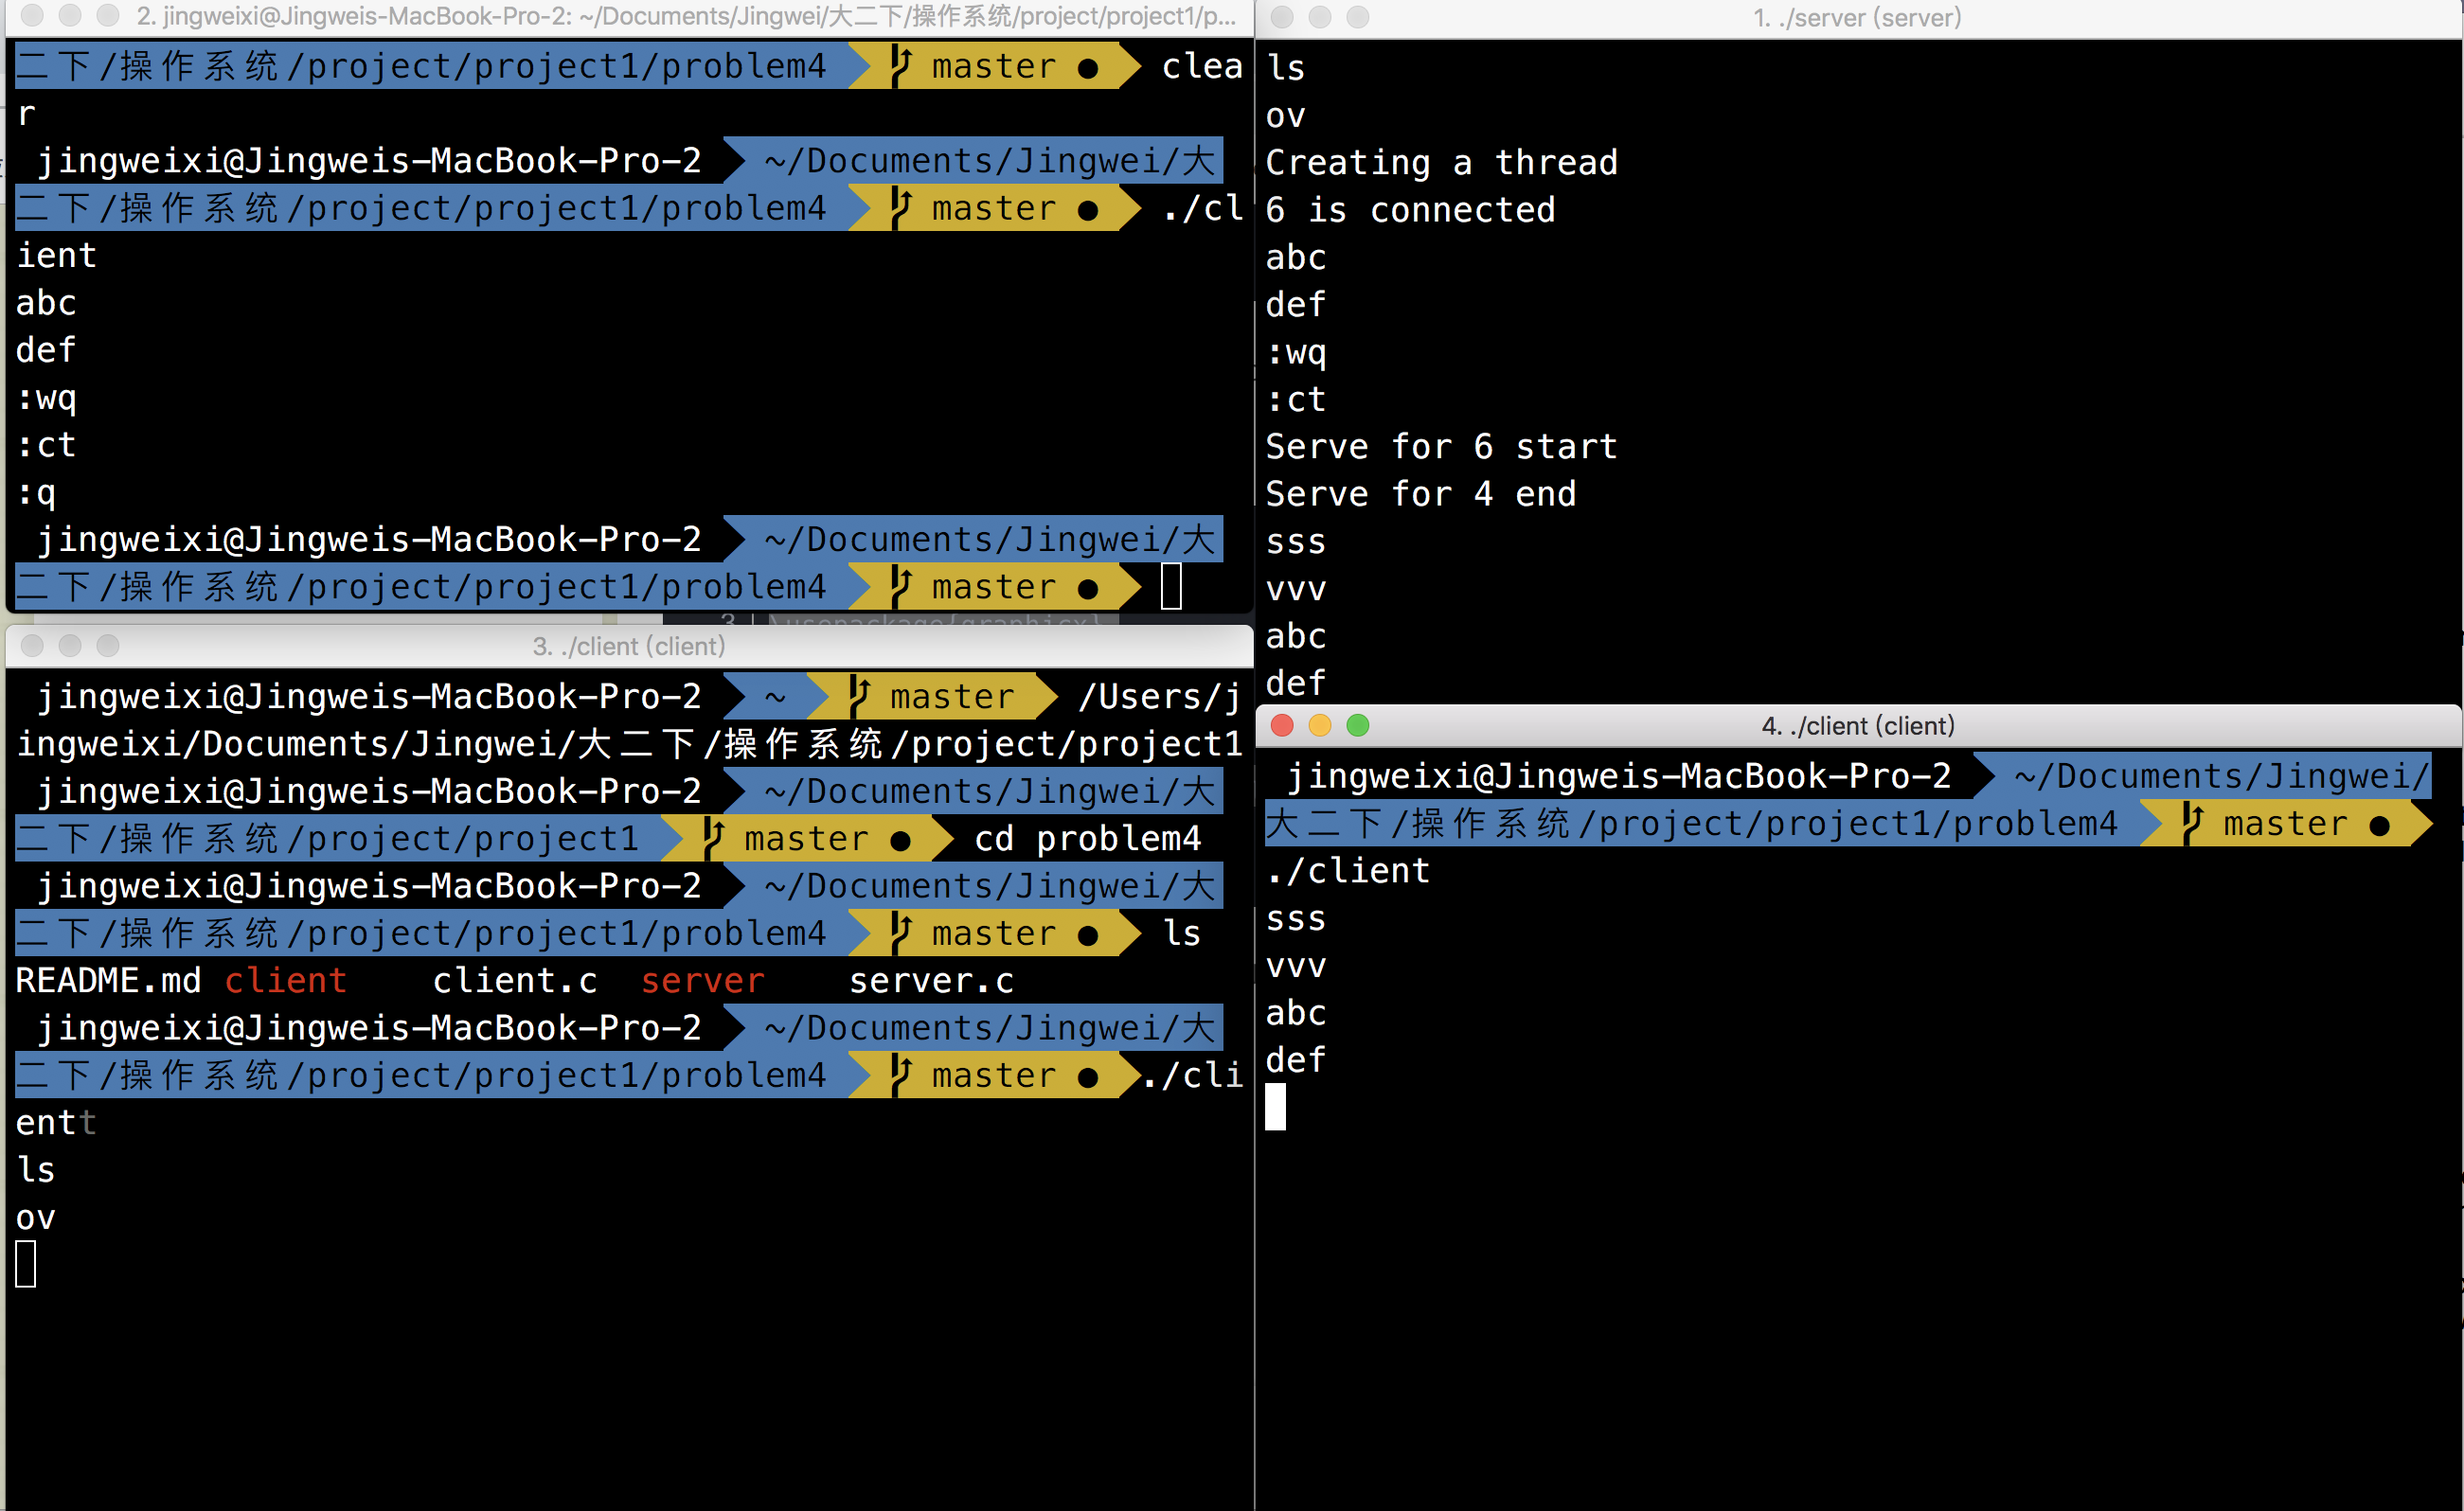
\includegraphics[scale=0.3]{2.png}

\end{document}